\documentclass[11pt,twocolumn]{article}
\usepackage{graphicx,url,placeins,algorithm,subcaption, algorithmic,lipsum,amssymb,amsmath,float}
\usepackage[hidelinks]{hyperref}
\usepackage[titletoc]{appendix}
\usepackage{pdfpages}
\usepackage{listings}

\usepackage{breqn}

 %\renewcommand{\familydefault}{\sfdefault}

\usepackage{natbib}

\makeatletter
\let\@texttop\relax
\makeatother
\topmargin-0.32in
\textheight22.2cm

\usepackage{layout}
%\usepackage[font=small,labelfont=bf]{caption}
\usepackage[utf8]{inputenc}
%\graphicspath{{figures/}}
%\setlength{\voffset}{0in}
%\setlength{\headsep}{1pt}
%\addtolength{\textheight}{2cm}
%\setlength{\footskip}{5pt}
%
\begin{document}
\title{\vskip -4em Cumulus}   % type title between braces
\author{Andreas Valter, andva287@student.liu.se \\
Johan Beck-Nor\'{e}n, johbe559@student.liu.se}
\date{\today}    % type date between braces
\maketitle
\begingroup
% \let\clearpage\relax % Removes blank page before include

\begin{abstract}

\end {abstract}

\section{Background}
Real time rendering is something that has been almost exclusive to game development where new games demands a higher quality to convince gamers to buy that game, instead of others.
This industy leads to a demand for better computer components that allows the games to run smoothly which leads to a decrease in cost for these components as the demand goes up.
This results in cheap and fast components, highly tuned for the computations that games does.
Other industries that faces similar problems can reap the benefits and this is something that is especially applicable for the visual effects (VFX) industry.

The general workflow for a VFX company is to create scenes with models that are interacting with each other and real people.
While working the artists handles simple place holders that represents the final output and when they think they are done, they push the work to a rendering farm for rendering.
To render a scene takes time, these super computers needs to calculate how the light interacts in the scene, resulting in a high quality estimation of how the scene looks.
But the interface that the artists are working with is often of much less quality then the final output, something that moves testing from the local computer to the farm.
This would lead to a real time output for changes made to simulations and models.

Therefore a lot of resent research has been aimed at moving work from the CPU that is not optimized for graphics computations to the GPU which converts application from offline to real time rendering.

\subsection{Maya and Viewport 2.0}
Viewport 2.0 is one of many indications that the VFX industry is moving towards incorporating real time renderings into the artist workflow.
One of the most commonly used tools for doing virtual effects is Autodesk Maya.
Maya is a 3D animation software that incorporates many of the tools needed to model, rig and simulate.
A example of how it looks when working inside Maya is show in \autoref{fig:mayaviewport} with menus on the sides and the viewport in the centre.
The fact that it is easily extendible makes it a good tool base for VFX companies which they can extend to fit their workflow.
It is inside this application that Viewport 2.0 exists.
It was introduced in the 2012 version of Maya to allow for custom drawing, shading and effects by creating a new rendering architecture in Maya.

\begin{figure}[ht]
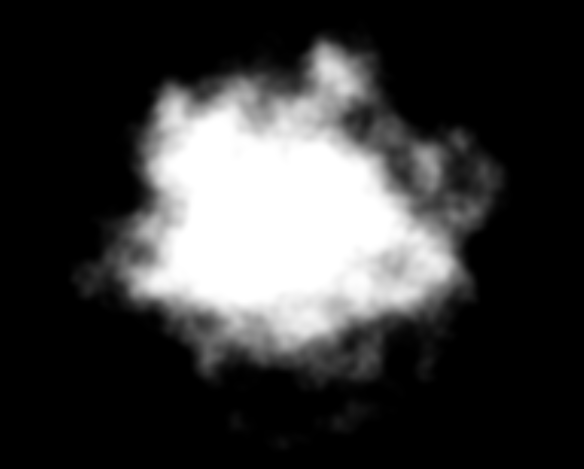
\includegraphics[width=0.5\textwidth]{figures/cumulus_slice.png}
\caption{A single ``slice `` of the noise generated cloud density data.}
\label{fig:cloud_slice}
\end{figure}

\section{Implementation}
\subsection{Density data generation}
The density data for the cloud volume was rendered using Simplex noise. Simplex noise is a further developed version of ``regular'' Perlin noise introduced by Ken Perlin. We created the cloud shape from a basic unit sphere, and then displacing the surface of the sphere by using a number of simplex noise contributions of differenct frequencies. The noise functions where weighted after frequency summed to form the final displacement amount.
\begin{figure}
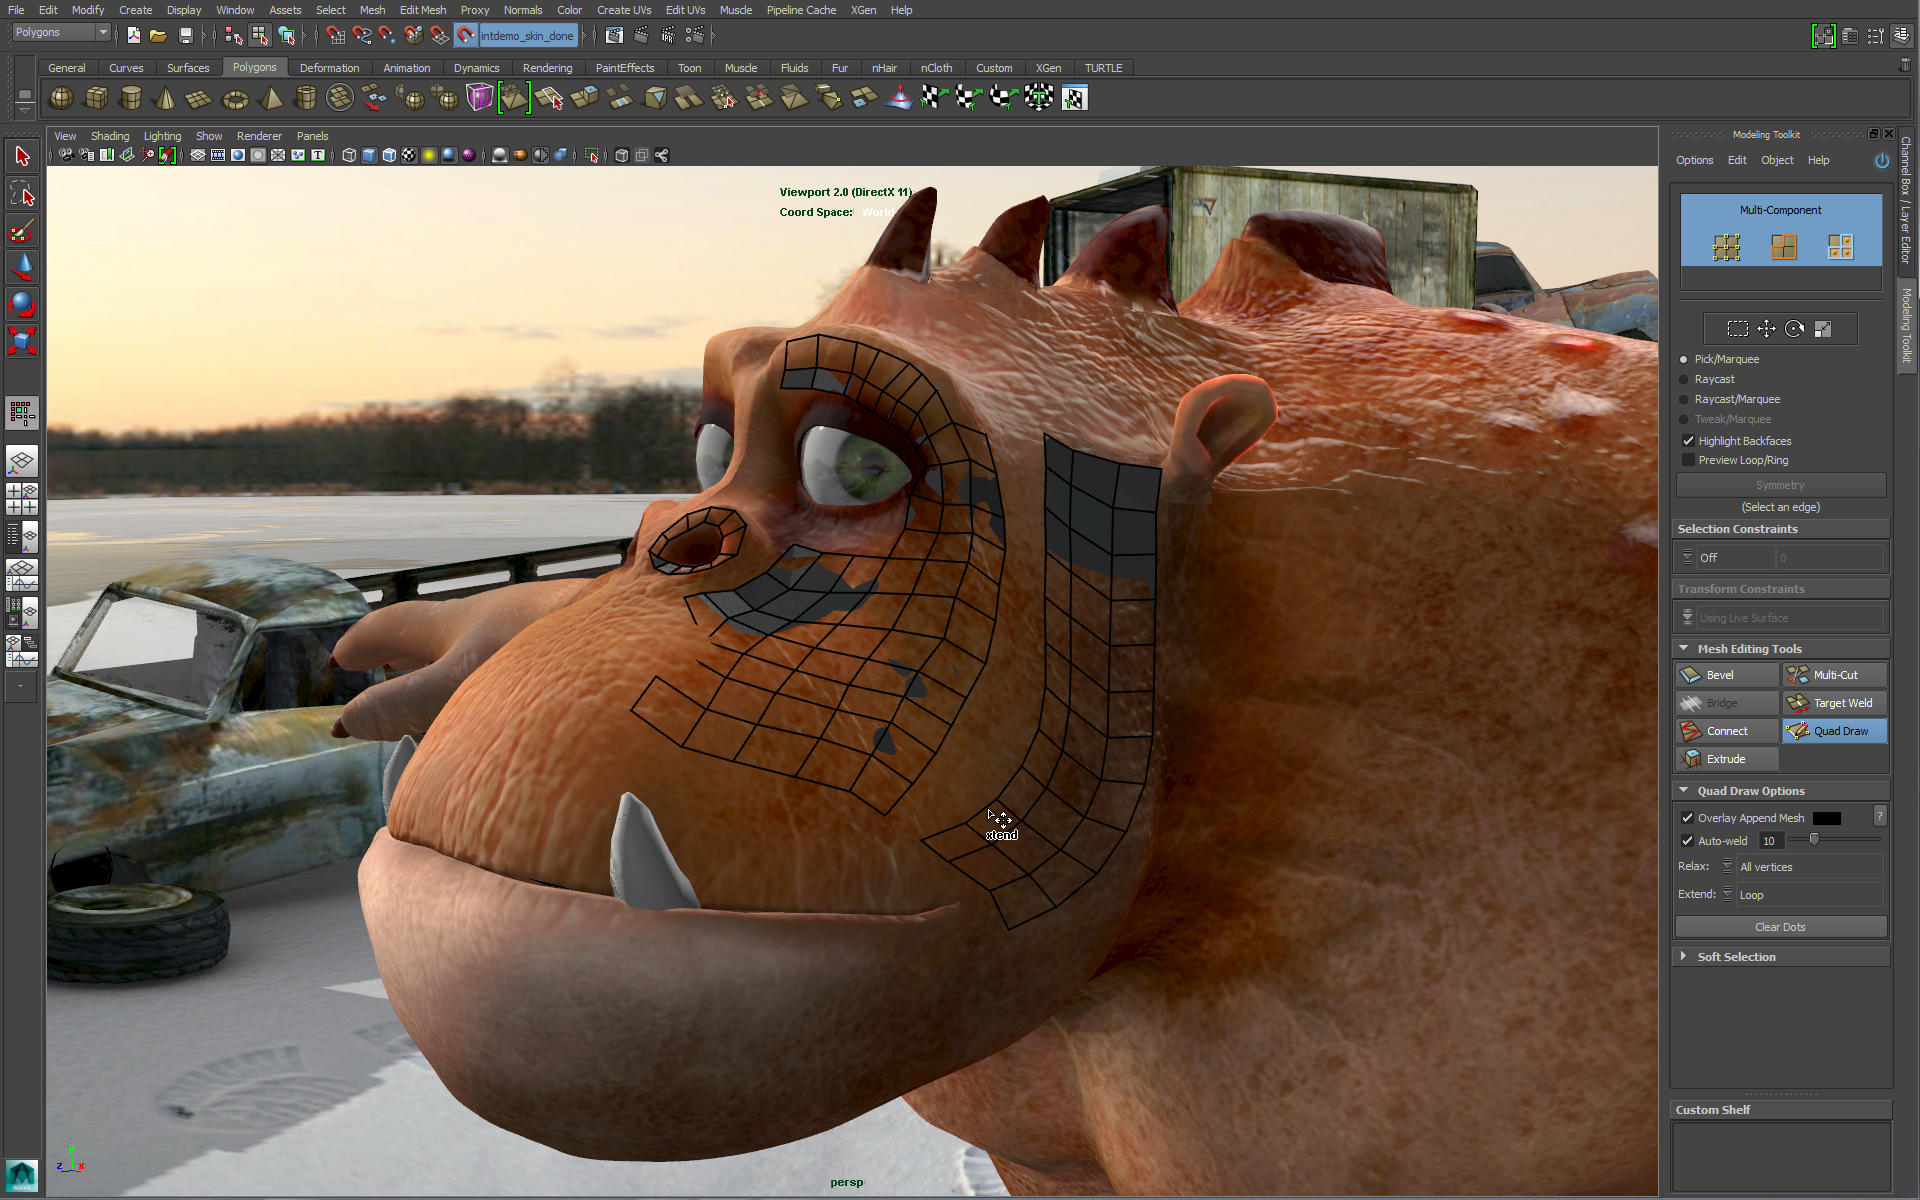
\includegraphics[width=0.49\textwidth]{figures/maya.png}
\caption{Example of Autodesk Maya UI and the viewport in action. Taken from http://area.autodesk.com/products/features/extensionmaya}
\label{fig:mayaviewport}
\end{figure}
\subsection{Design}
For the implementation we knew that the final goal was a plugin for Maya.
But for development purposes we wanted a faster and more intuitive way to test run our code without having to restart Maya and load up our plugin each time.
Instead separated the code into two layers. The bottom layer is the core where the meat of the implementation is located. It is in this layer we generate our volume density data, performe the ray marching etc. About the core layer we have two modules, on for rendering with OpenGL and one for rendering to a Maya plugin. The OpenGL module uses a GL viewport for rendering and requires no external software or installs other that the required GL libraries. This provided us with a fast way to develop and test our code thoughout the project. The workflow would be to develop using the OpenGL module and once the results looked as intended in the GL viewport we could compile it to a Maya plugin.
\subsection{Ray Marching}
A volume data set is simply numbers representing density values at some point in the volume space.
In our implementation the volume data is stored as a 3D texture.
Together with GLSL shaders this allows for the use of fast hardware trilinear interpolation of values for arbitrary points within the volume. To determine the final color for a pixel on the screen we use ray marching to sample the volume.
The most simple case is a volume set aligned with the camera viewing direction.
This would only require samples to be taken along a ray aligned with the volume axes.
Density values in the volume are sampled along the ray at sample points with a uniform spacing and the final density for the pixel is a sum of all the sampled density values.
This is the implementation we used in this project.
\\
A method to allow for interactive camera positioning around the volume used extensively in scientific visualization is a method using a color cube.
A uniform cube is rendered first using front face culling and then using back face culling.
For each pixel the position is stored in a frame buffer object texture in a first rendering pass.
For the volume rendering pass these textures are used to determine a ray direction by comparing the values stored in the front face and back face textures for each pixel. From this we retrieve a ray origin position and a ray direction, which is then used to sample the volume in the same uniform fashion as described in the previous paragraph. An attempt was made to use this method in our implementation, but we did not succeed in using frame buffer objects together with the Maya Viewport 2.0.

\begin{figure}
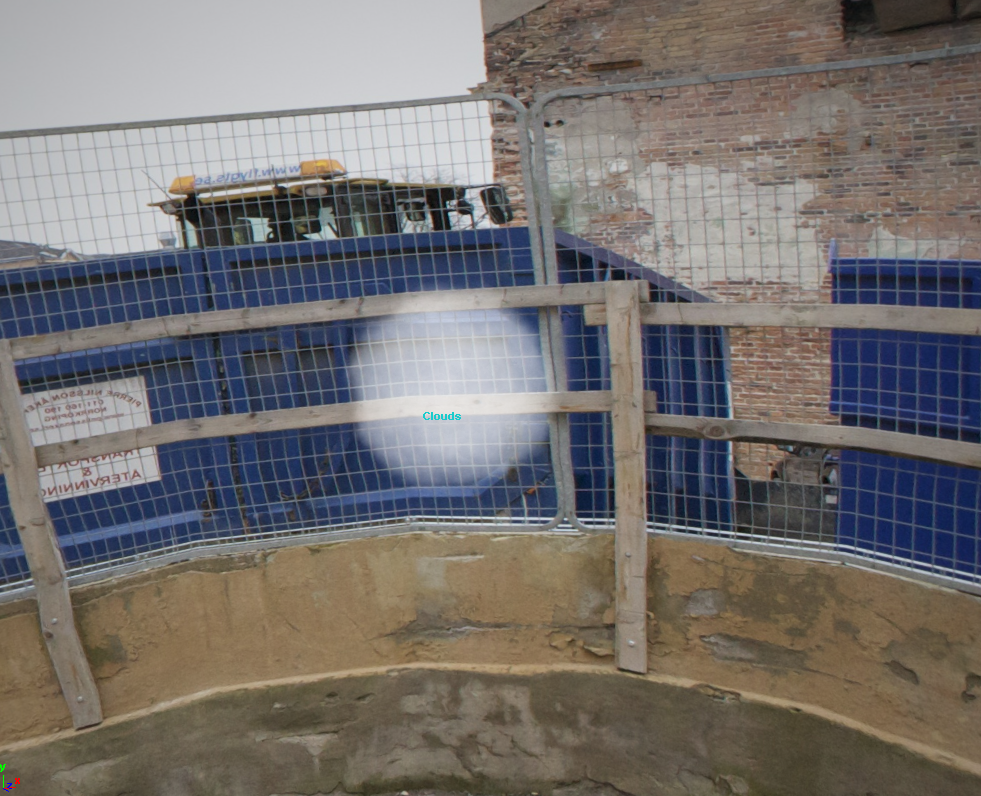
\includegraphics[width=\textwidth]{figures/cloudlol.png}
\caption{Our cloud plugin displayed in realtime in the Maya Viewport 2.0.}
\label{fig:mayaviewport_final}
\end{figure}

\endgroup
\newpage
\bibliographystyle{abbrv}
\nocite{*}
\bibliography{bibl}

\end{document}